\documentclass[tikz]{standalone}
\usepackage{amsmath}
\definecolor{morange}{RGB}{255,127,14}
\definecolor{mblue}{RGB}{31,119,180}
\definecolor{mred}{RGB}{214,39,40}
\definecolor{mpurple}{RGB}{148,103,189}
\definecolor{mgreen}{RGB}{44,160,44}

\immediate\write18{julia --project="../.." rosenbrock_plot.jl}

\newcommand{\pro}{\ensuremath{\mathcal{P}}}
\newcommand{\rec}{\ensuremath{\mathcal{R}}}

\begin{document}
\begin{tikzpicture}[
    squarednodeF/.style={circle, draw=black!60, fill=mpurple!5, very thick, minimum size=10mm},
    squarednodeR/.style={rectangle, draw=black!60, fill=mblue!5, very thick, minimum size=5mm},
    ]
    %Nodes
    \node      (fig)                              {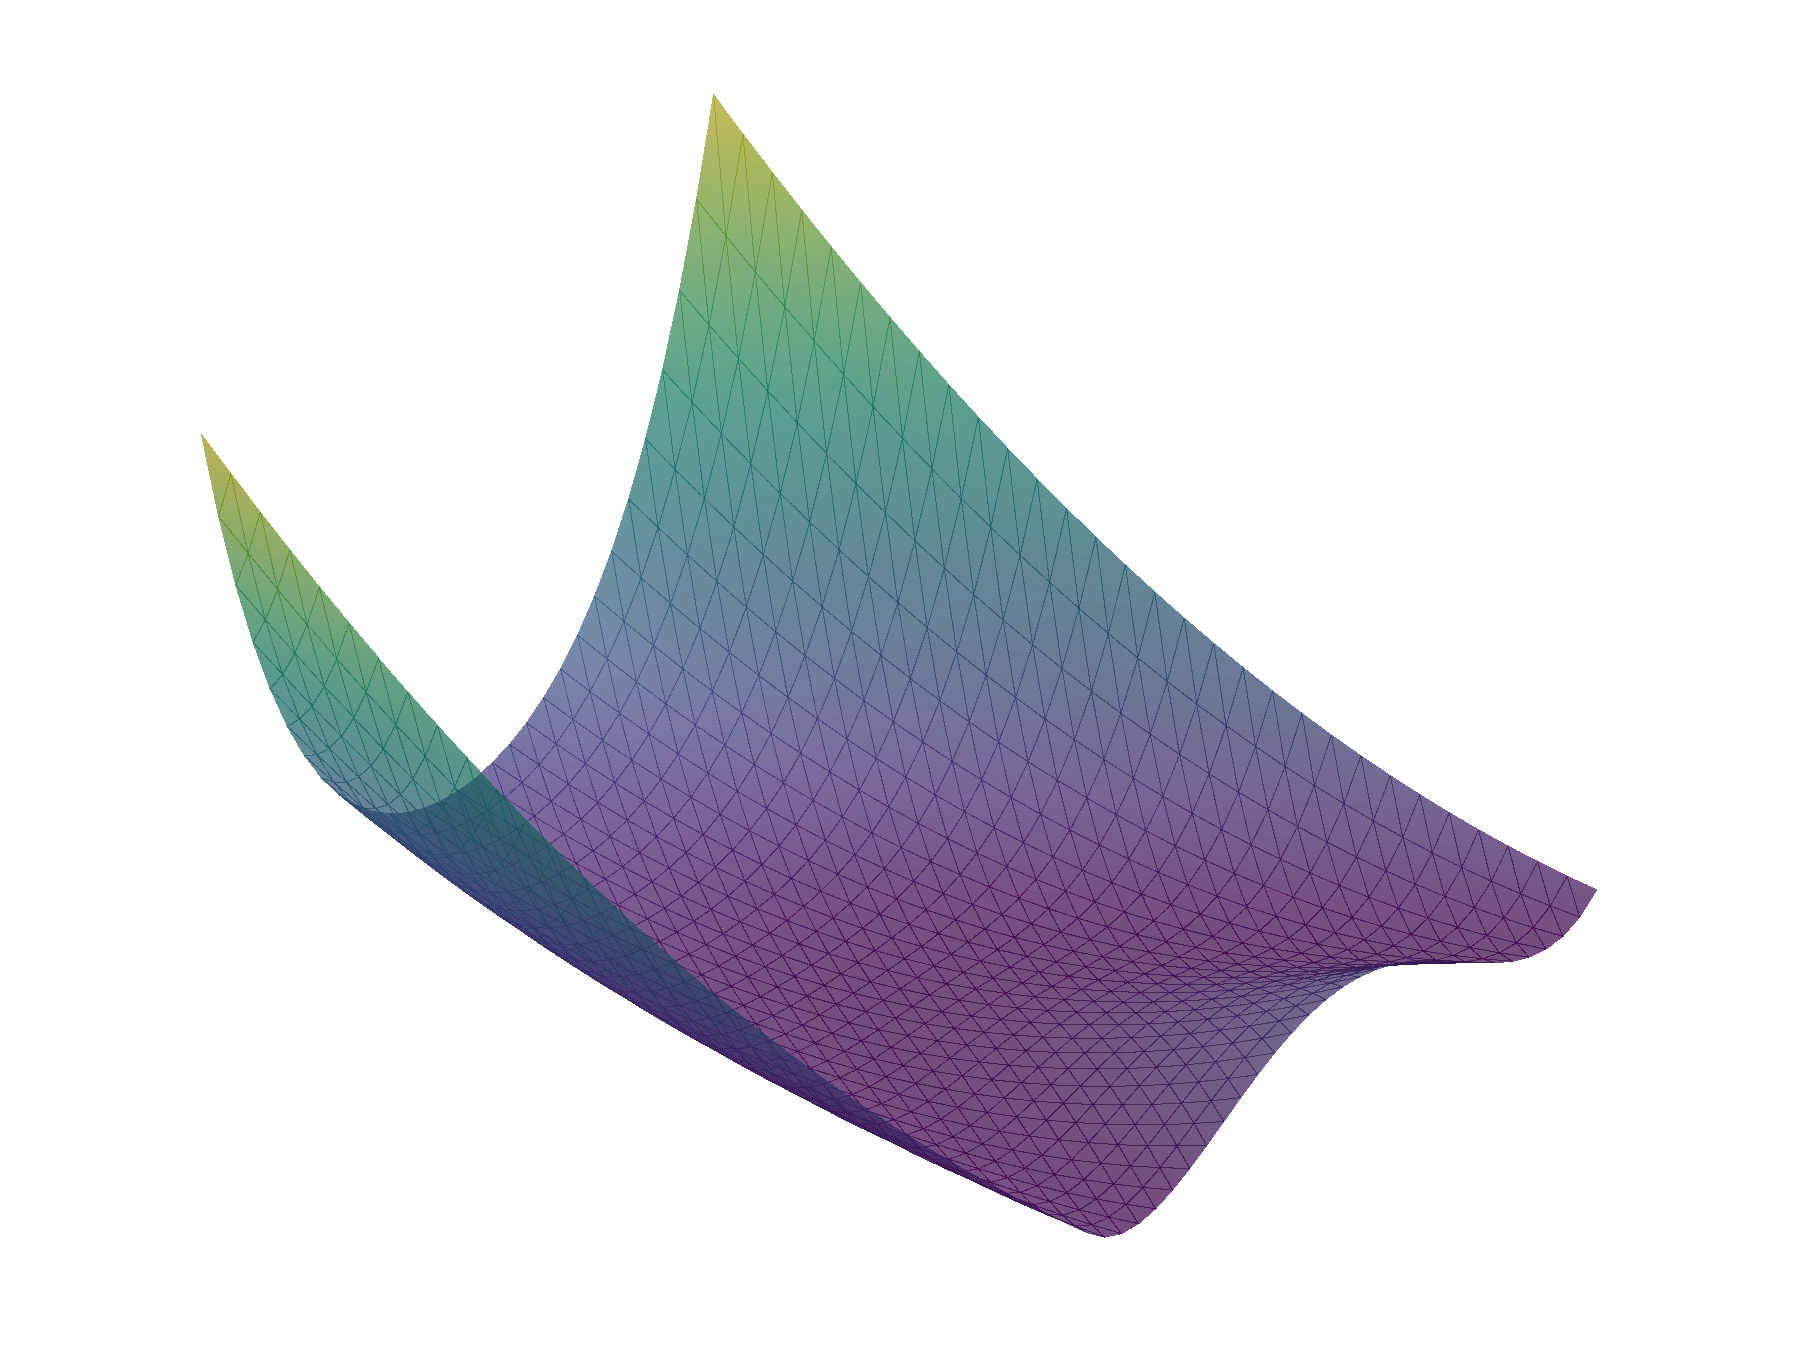
\includegraphics[width=.3\textwidth]{rosenbrock_naked}};
    \coordinate[below of=fig, yshift=.1cm] (gr_plot);
    \node[squarednodeR]        (samples)       [below of=fig, yshift=-2cm] {$\begin{aligned} \begin{pmatrix} x^{(1)} \\ y^{(1)} \\ z^{(1)} \end{pmatrix},  \begin{pmatrix} x^{(2)} \\ y^{(2)} \\ z^{(2)} \end{pmatrix}, \cdots, \begin{pmatrix} x^{(\mathtt{np})} \\ y^{(\mathtt{np})} \\ z^{(\mathtt{np})} \end{pmatrix}\end{aligned}$};
    \node[squarednodeR]      (reduced1)       [right of=samples, xshift=6cm] {$\mathcal{NN}$};
    \node        (fig2)       [above of=reduced1, yshift=2cm] {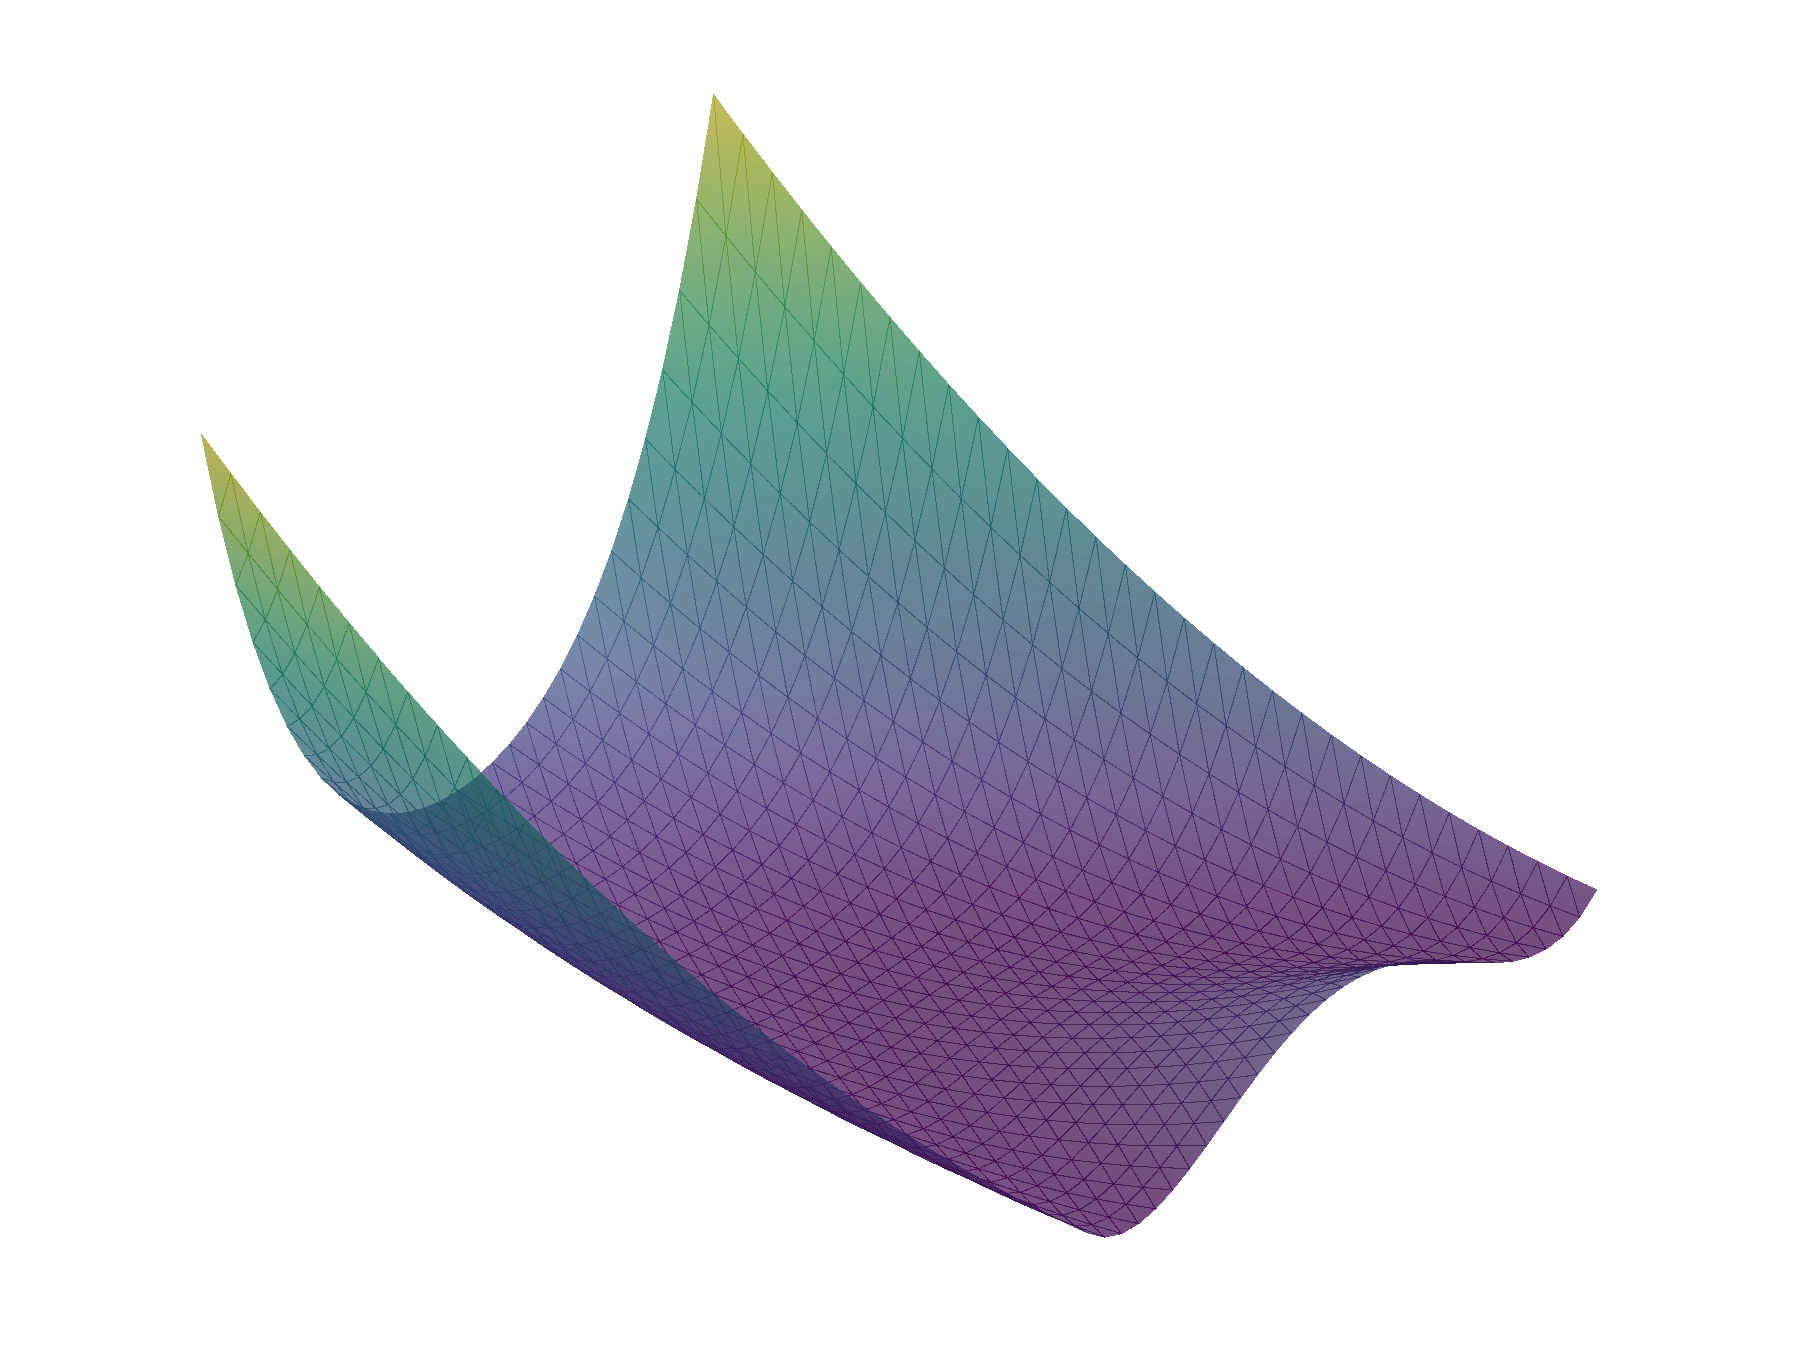
\includegraphics[width=.3\textwidth]{rosenbrock_naked}};
    \coordinate[below of=fig2] (gr_plot2);

    %Lines
    \draw[->, mred] (gr_plot) to node[right] {sampled points (given)} (samples.north);
    \draw[->] (samples.east) to node[above] {build neural network} (reduced1.west);
    \draw[->, mblue] (reduced1.north) to node[left] {sample points} (gr_plot2);
    \end{tikzpicture}
\end{document}
